\section{Valg av løsning}
Dette kapittelet handler om valg av løsninger for oppgaven. Valg av posisjonssystem for prosjektet er i fokus.

\subsection{Systemkrav}
Systemkrav for valg av posisjonssystem
\begin{itemize}
\item Systemet bør være motstandsdyktig mot interferens
\item Systemet skal ikke interferere andre sendere/mottakere på dronen
\item Posisjon i x/y planet skal være mer nøyaktig enn GNSS (uten RTK), sikter på system med nøyaktighet under 1m.
\item Systemet skal være innenfor regelverk for sendestyrke og frekvenser
\item Systemet skal kunne beregne lokal posisjon 
\item Rekkevidden til systemet bør være over 30meter
\end{itemize}

\subsection{Forslag til andre posisjonsmetoder enn UWB}
Bachelor oppgaven er i samarbeid med bedriften Kongsberg, bedriften har ønsket at prosjektet skal teste UWB som posisjonssystem. Likevel ble andre teknologier vurdert av gruppen for alternative løsninger. System som gir ut posisjon i koordinater ble vurdert og system som finner avstand til objekt slik som lidar og stereokamera ble ikke vurdert. 

\begin{figure}[htp]
    \centering
    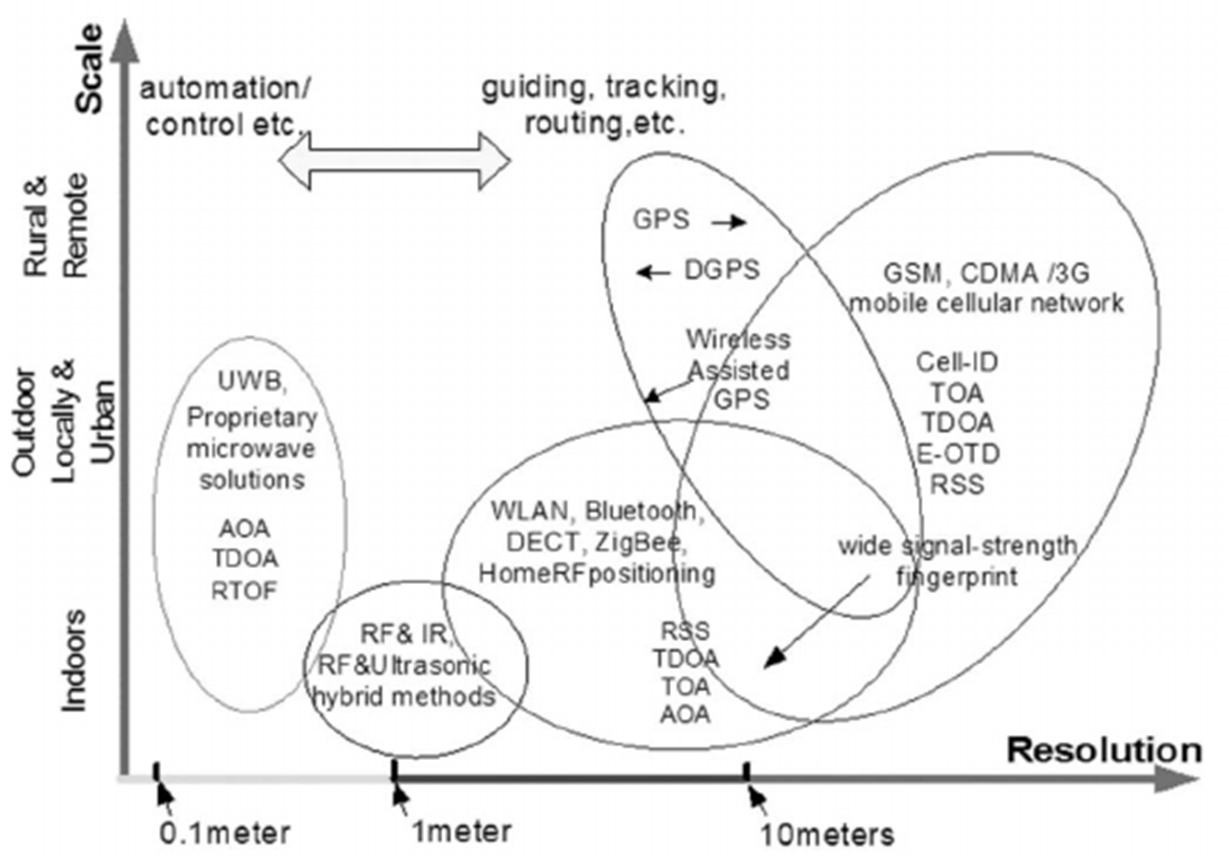
\includegraphics[width=0.7\columnwidth]{figures/posisjoneringssystemer}
    \caption{Sammenlikning av posisjoneringssystemer.}
    \label{fig:posisjoneringssystemer}
\end{figure}

\subsection{Kamera triangulering}

\begin{figure}[htp]
    \centering
    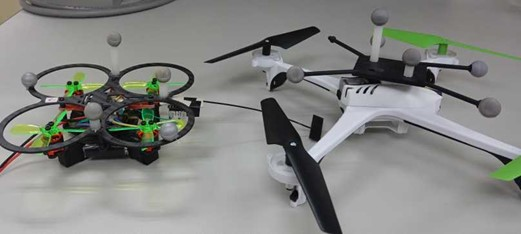
\includegraphics[width=0.7\columnwidth]{figures/kameratriangulering}
    \caption{Droner for kameratriangulering.}
    \label{fig:kameratriangulering}
\end{figure}

Kamera triangulering bruker flere kamera for å triangulere posisjonen til ett eller flere objekt. På objektet som skal spores plasseres flere markører. Slik kan man finne posisjonen og rotasjonen. Denne teknologien er mye brukt i filmproduksjoner og spillutvikling.
Kamera triangulering kan være veldig nøyaktig. Systemet Optitrack beskriver oppløsningsavviket på millimeternivå.  Disse systemene kommer ofte med en høy pris, som er utenfor prosjektets budsjett. Rekkevidden til systemene er og litt kort til prosjektets anvendelsesområde, og utendørsbruk kan være krevende. 

\subsubsection{Bluetooth, Zigbee og Wifi}
Denne teknologien baserer seg på signalstyrke for å beregne posisjonen. Oppløsningen på posisjonen til vil ligger i meterområdet bluetooth (ca 1-5m) og Wifi(ca5-20), det vil være for unøyaktig for prosjektets anvendelsesområde siden det er mer unøyaktig enn GNSS kan være. 
Denne teknologien bruker frekvenser innenfor 2.4ghz og 5.8ghz De fleste droner bruker allerede disse frekvensene for kommunikasjon, her vil sendingen kunne forstyrre hverandre.  

\begin{figure}[htp]
    \centering
    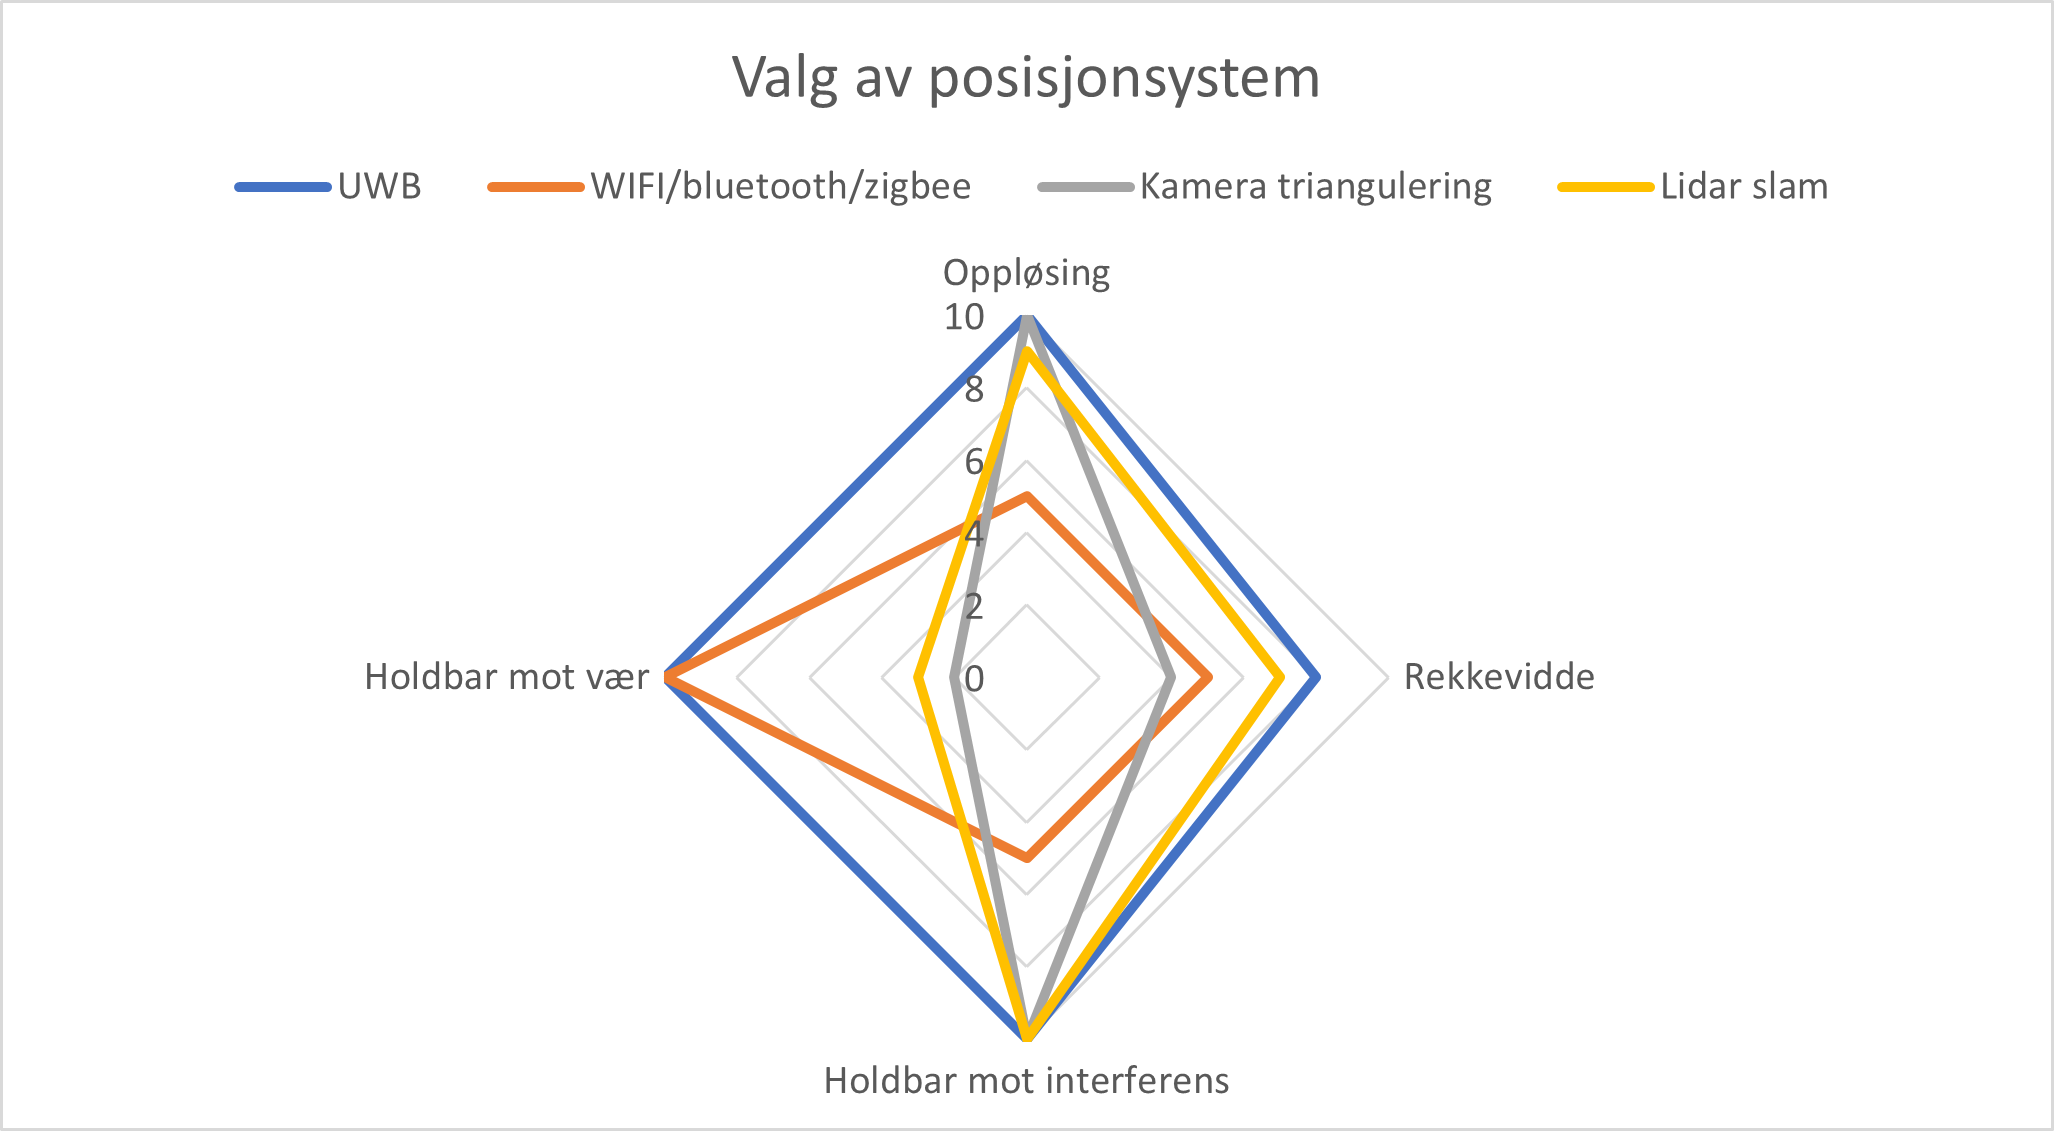
\includegraphics[width=0.7\columnwidth]{figures/valgavsystem}
    \caption{Valg av system.}
    \label{fig:valgavsystem}
\end{figure}

\subsubsection{UWB}
I sammenligningen med de andre posisjonssystemene slår gruppen fast at UWB vil kunne fungere godt for anvendelsesområdet for oppgaven. 

\subsection{Valg av UWB system}
For valg av UWB-system var det 3 forskjellige systemer som ble vurdert.

\subsubsection{DWM100}

\begin{figure}[htp]
\centering
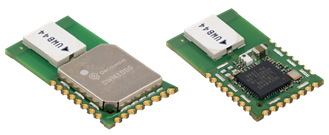
\includegraphics[width=0.5\columnwidth]{figures/dwm100}
\caption{DWM100.}
\label{fig:dwm100}
\end{figure}

Denne UWB modulen består av UWB sensoren DW1000 som er brukt i flertallet av UWB system. For prosjektets bruk sammen med en drone er det nødvendig å lodde modulen til en mikrokontroller. Det trengs og en løsning for å gi strøm til sensorene. 
For å bruke DWM1000 til å finne posisjon er det nødvendig med programvare som triangulerer signalene fra modulene, det finnes ingen tilgjengelig programvare for dette slik at mye arbeid i bacheloren ville gått til programmering. 

\subsubsection{DWM1001}

\begin{figure}[htp]
\centering
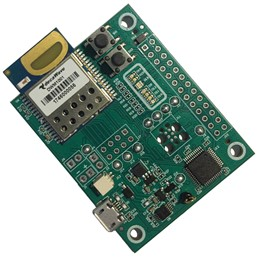
\includegraphics[width=0.4\columnwidth]{figures/dwm1001}
\caption{DWM1001.}
\label{fig:dwm1001}
\end{figure}

DWM1001 består av sensor/mottaker DW1000, i denne modulen er mikrokontroller inkludert, slik det er lite arbeid med oppkobling. 
Slik som DWM1000 vil det være mye arbeid med å programmere systemet til posisjonsbruk. 

\subsubsection{POZYX}

\begin{figure}[htp]
\centering
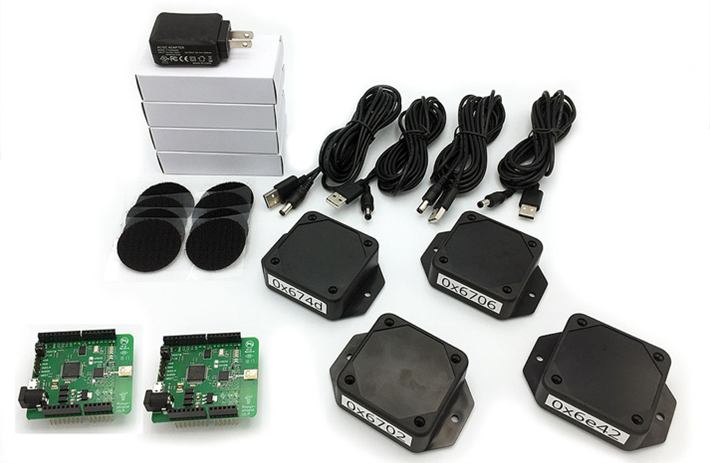
\includegraphics[width=0.7\columnwidth]{figures/creatorkitlite}
\caption{Pozyx creator kit lite.}
\label{fig:creatorkitlite}
\end{figure}

Pozyx systemet består av anker og tags som inneholder mikrobrikken Dw1000.  Creator kit Lite kommer med 4 anker og 2 tags. Dette systemet kommer med programvare og har god dokumentasjon for bruk med egen programvare.   

For å velge hvilket system gruppen skulle bestille ble ulike fakturer vurdert. Figur \ref{fig:valgavsystem2} demonstrerer de ulike faktorene.  Valget falt da på POZYX systemet da det passet godt til vår oppgave, det skal være lett å sette opp og har mye dokumentasjon. 
Det at POZYX systemet har ferdig programvarer og bibliotek passer godt til oppgaven, da oppgaven til prosjektet er ikke å programmere ett UWB-system fra grunnen, men det er å forske på hvordan UWB vil fungere i bruk med droner. 

\begin{figure}[htp]
\centering
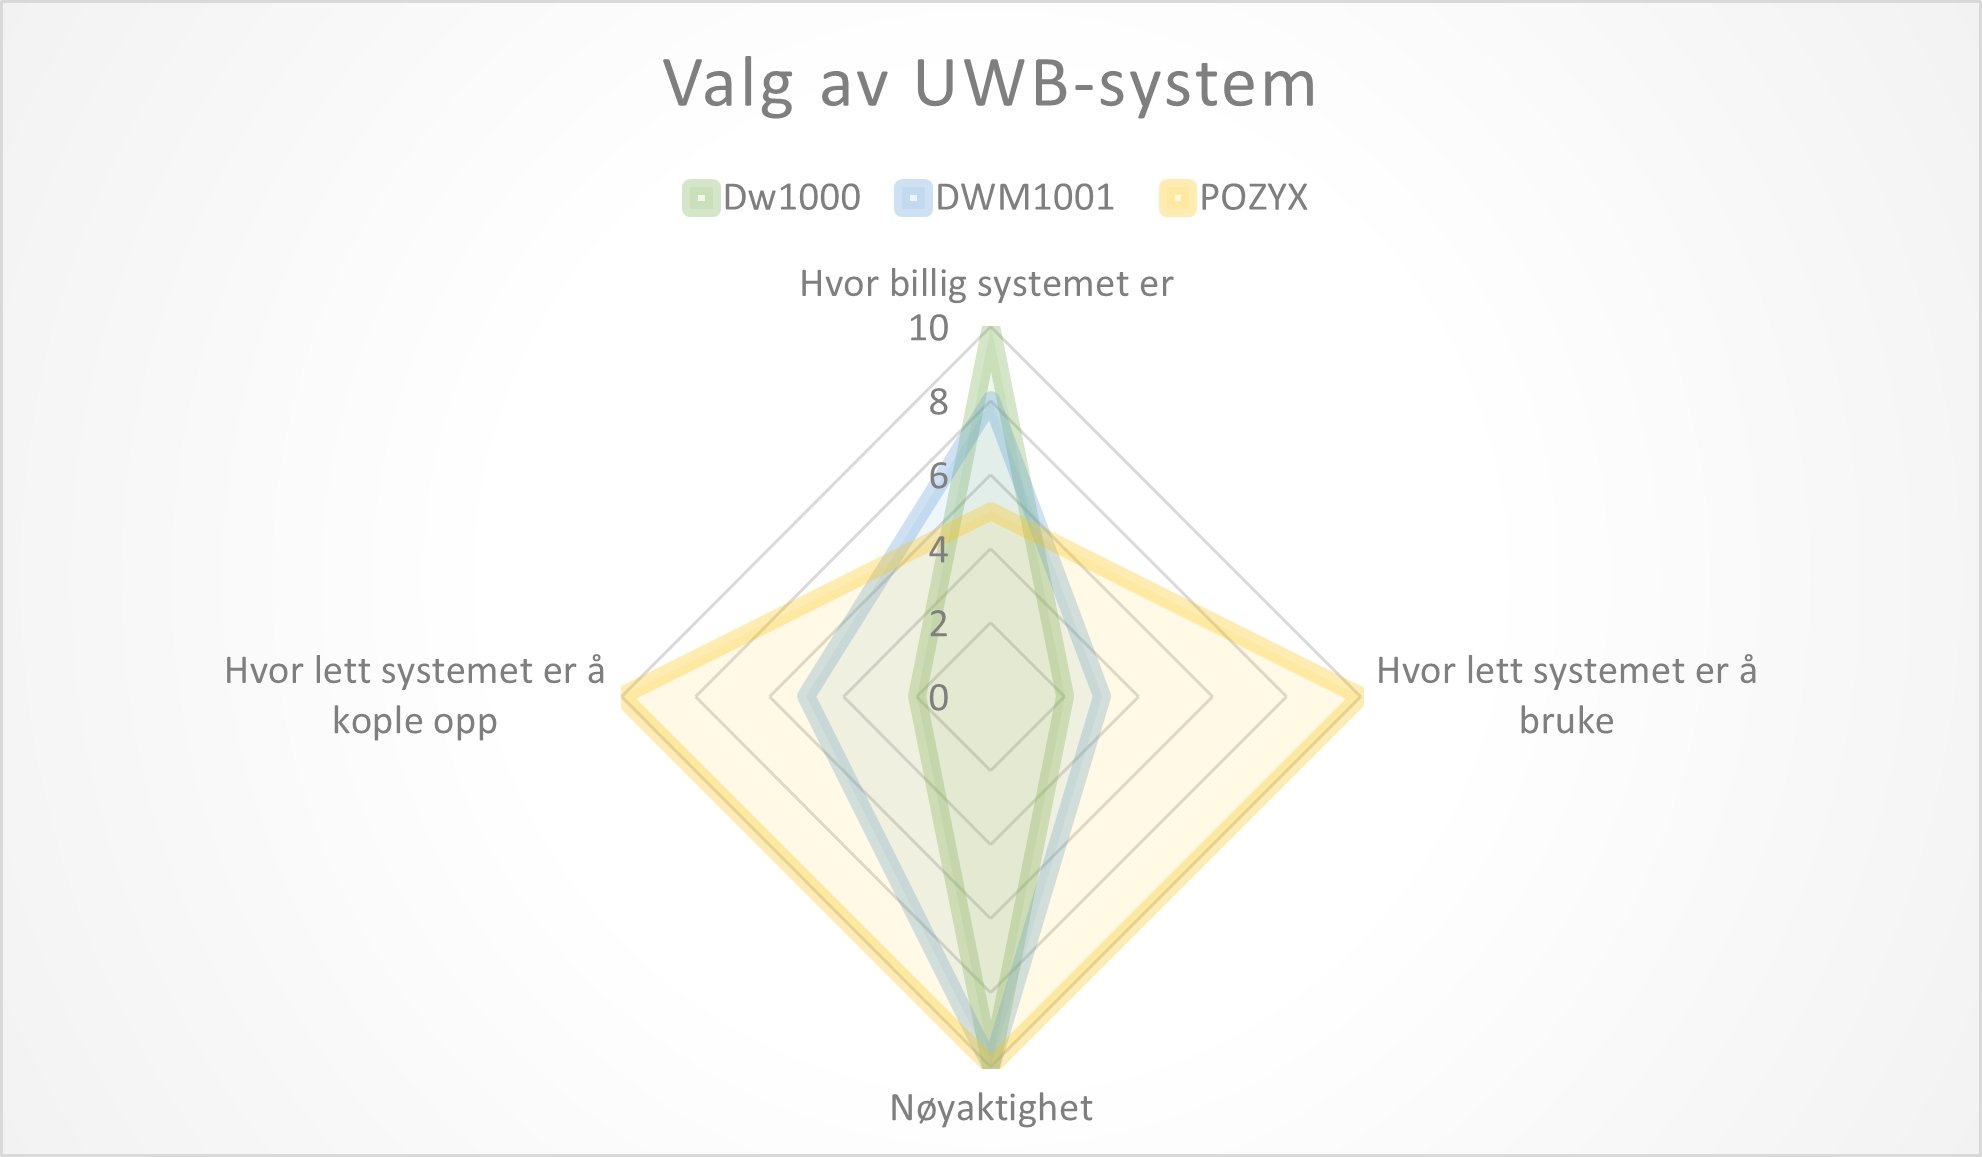
\includegraphics[width=0.7\columnwidth]{figures/valgavsystem2}
\caption{Valg av UWB system.}
\label{fig:valgavsystem2}
\end{figure}

\subsection{Valg av platform}

For å knytte prosjektet opp mot droneteknologiutdanningen har gruppen bestemt seg for å bruke quadrotor (drone) for prosjektet. Om prosjektet fungerer godt med enn drone, vil det sannsynligvis fungere godt for roveren til Kongsberg.
Erfaringer fra utendørsflyvninger i Tromsø der prosjektet utføres er at været er enn stor hindring, det ble derfor valgt å bruke en drone som er mulig å bruke innendørs. Valget ble å bruke en «racing» drone med propellerbeskyttere, som vist i figur \ref{fig:nakeddrone}. Denne dronen har løftekraften til å løfte sensorene som er nødvendig samtidig som den har liten størrelse. 

\begin{figure}[htp]
\centering
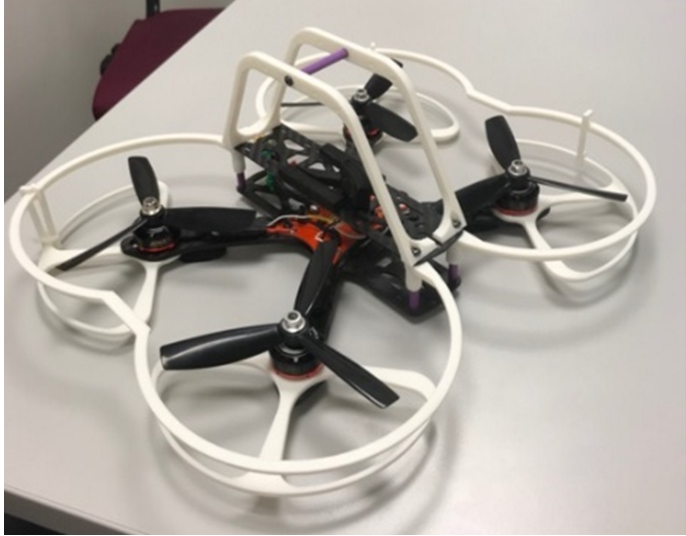
\includegraphics[width=0.6\columnwidth]{figures/nakeddrone}
\caption{Drone ramme med 3D-printet beskyttelse.}
\label{fig:nakeddrone}
\end{figure}

\subsection{Konsept}
Systemet består av et dronesystem med påmontert UWB-tag som kommuniserer med 4 UWB-anker. UWB-tagen regner ut avstandene til ankerene og sender dataen til flightkontrolleren. Målet er å bruke UWB-systemet til å kunne få dronen til å flyve ved hjelp av UWB-posisjon. Figur \ref{fig:konsept} viser dette.

\begin{figure}[htp]
\centering
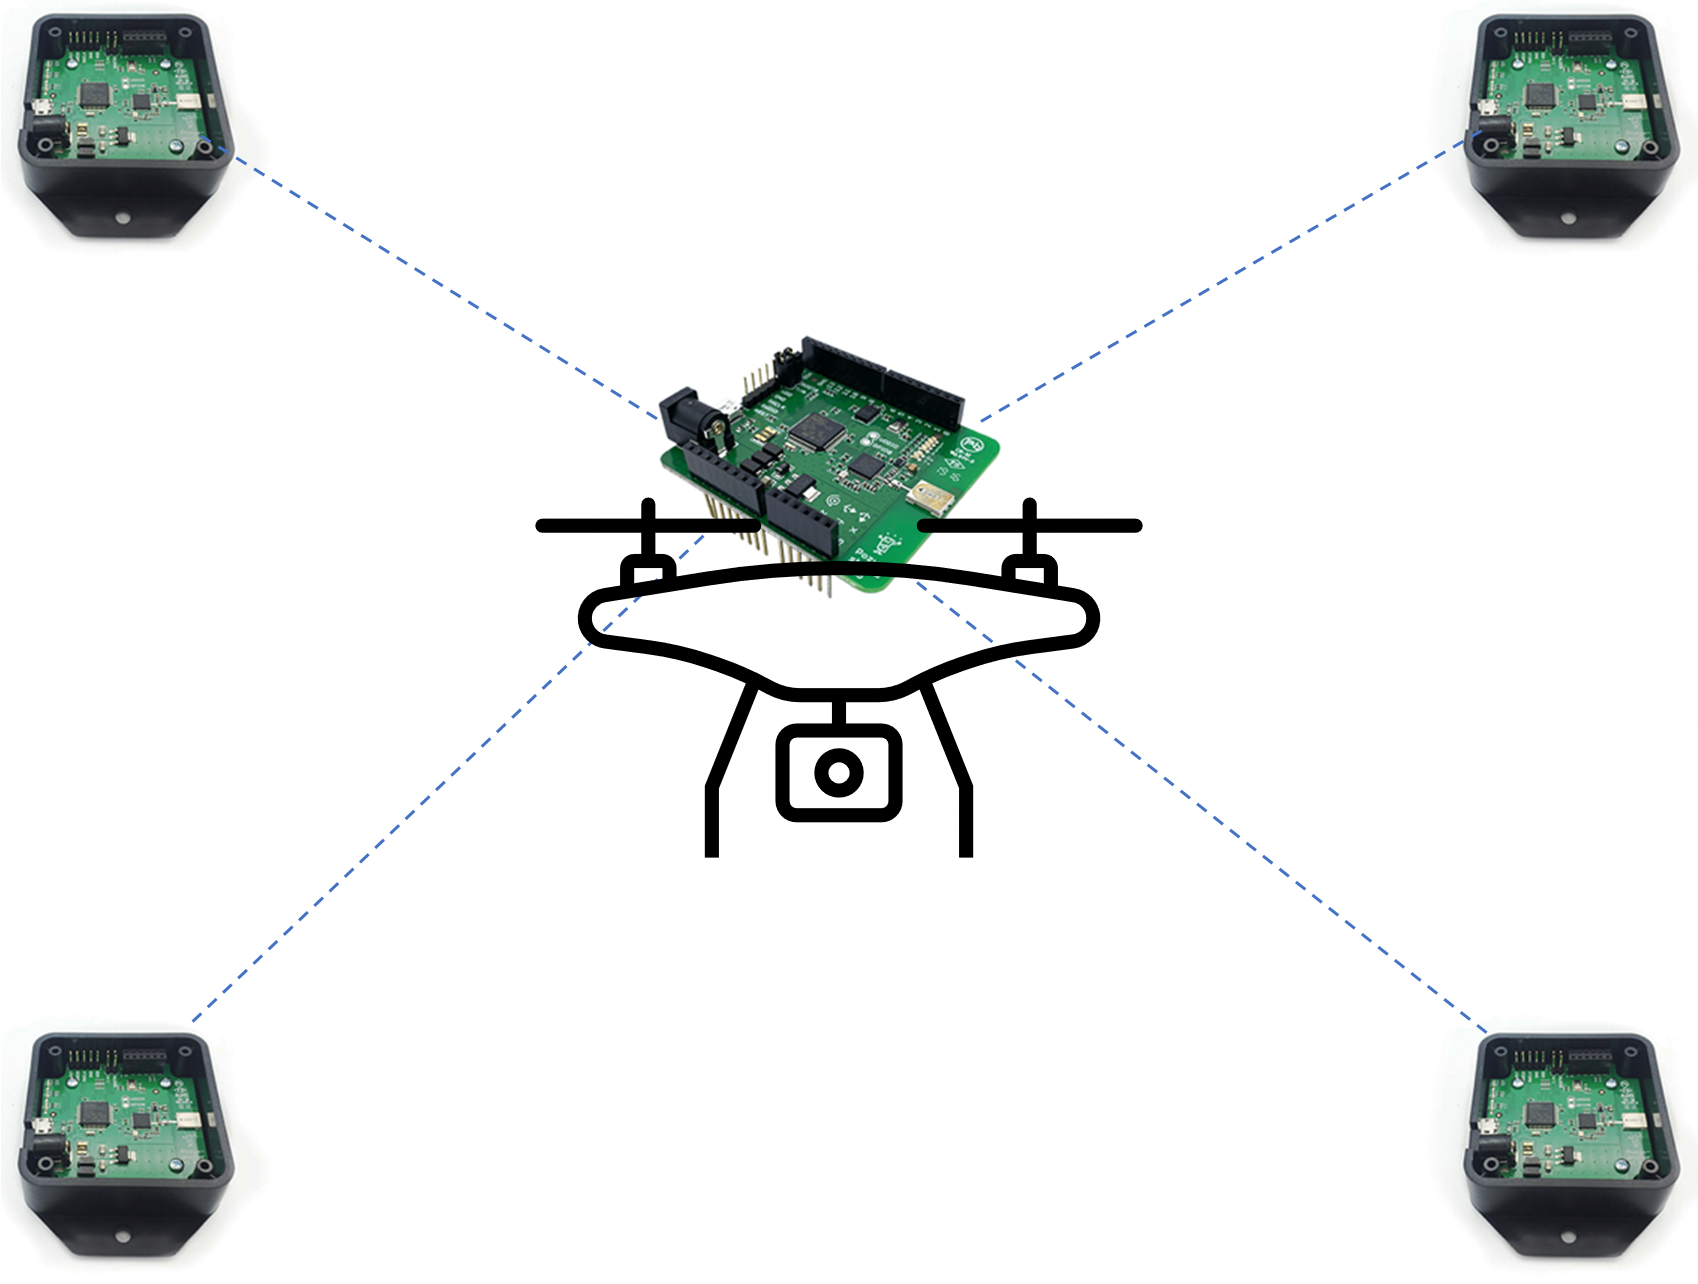
\includegraphics[width=0.5\columnwidth]{figures/konsept}
\caption{Posisjoneringskonsept.}
\label{fig:konsept}
\end{figure}

\subsubsection{Design av drone}
Det ble valgt å bruke en “racing” drone med 5 tommer propeller til prosjektet. For å få den sikker ble det vurdert at propellerbeskyttere måtte bli brukt. 

\subsubsection{3D-printede deler}
Det ble designet propellerbeskytter for å dekke både oversiden og undersiden av propellerbladet. Disse ble deretter festet på drone rammen. For å beskytte UWB-tagen ble det designet ett veltebur på oversiden av dronen. 
Batteriet ble plassert på undersiden av dronen på grunn av UWB-tagen sitter på toppen, for å beskytte batteriet mot harde landinger ble det designet landingsben for å ta imot kreftene. 
De 3d-printede delene ble printet i PLA plast, PLA vil kunne knekke i harde landinger eller krasj, men delene er designet for å kunne bli enkelt byttet ut.  Delene ble designet i Fusion 360. For å finne ut hvor delen vil kunne få svikt ble stressanalyseverktøyet til Fusion 360 brukt, som vist i Figur \ref{fig:stresstest}.

\begin{figure}[htp]
\centering
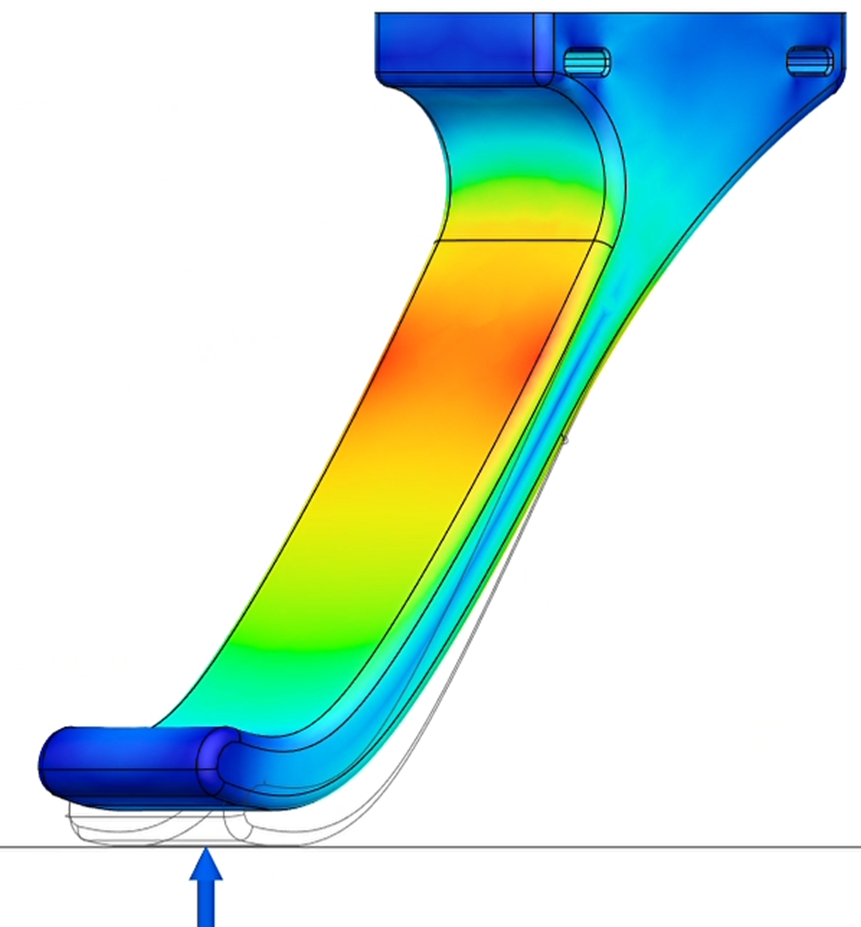
\includegraphics[width=0.4\columnwidth]{figures/stresstest}
\caption{Stresstest i Fusion 360}
\label{fig:stresstest}
\end{figure}

\subsubsection{Oppkobling av dronen}
Dronen består av flightkontroller, motorer, motorkontroller...

\subsubsection{UWB-tag til flightcontroller}
For å få data fra UWB-tagen til rett protokoll til ardupilot var det nødvendig med en mikrokontroller for å “oversette”. I figur\ref{fig:oppkobling} vises oppkoblingen fra UWB-tag t.v til mikrokontroller til flightkontroller. 
På mikrokontrolleren kjøres ett datascript som setter opp UWB-tag for å kunne kommunisere med ankerene ved å sette rette adresser til anker, samt hvor ankerene er plassert. Deretter regnes det ut avstand til hvert anker og koordinat til tag-en. For at flightkontrolleren skal forstå dette må det sendes på riktig protokoll som arduinokoden ordner.   

\begin{figure}[htp]
\centering
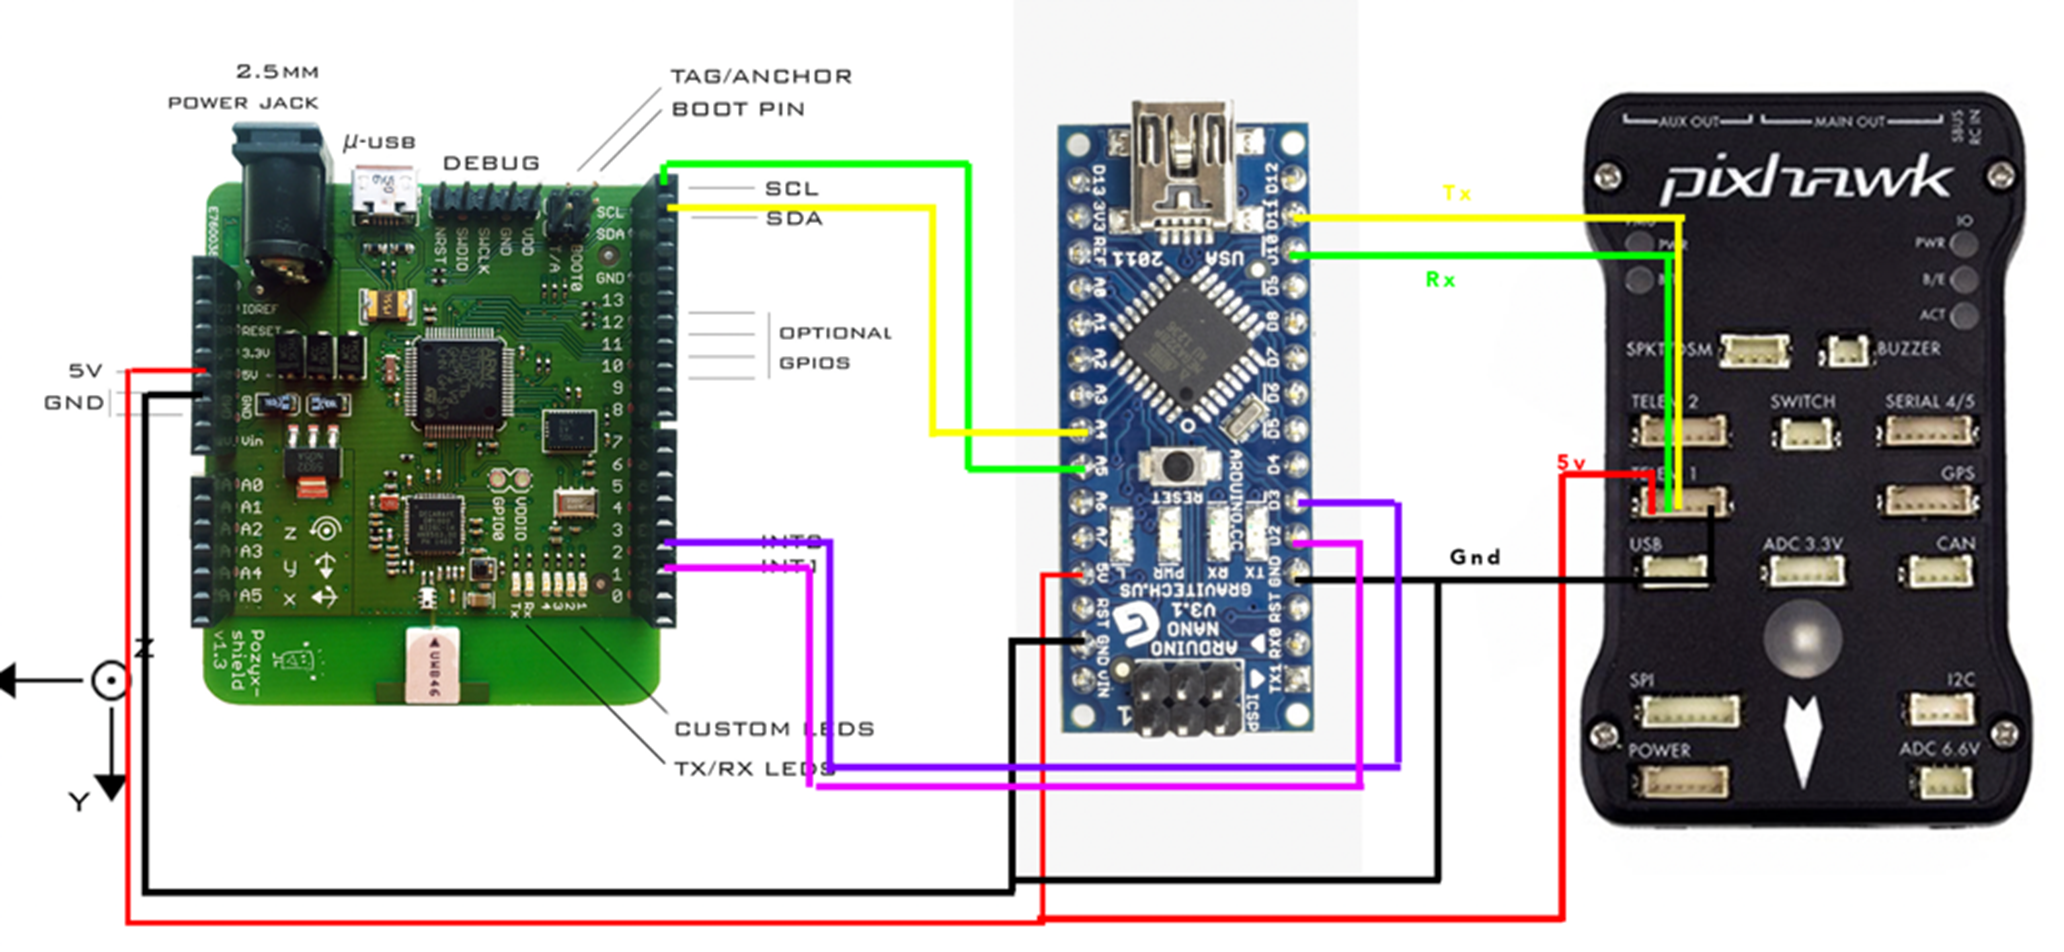
\includegraphics[width=0.7\columnwidth]{figures/oppkobling}
\caption{Oppkobling av "Oversetter" fra UWB-tag til flightkontroller.}
\label{fig:oppkobling}
\end{figure}

\subsubsection{Oppsett av anker}
For at UWB-tag-en skal kunne regne ut posisjonener den avhengign at ankerene er plassert rikig. Det er viktig at ankerene ikke beveger seg, har riktig orientasjon og riktig plasering. Ankerene trenger og strøm for å kjøre siden de svarer tag-en sine meldinger. 
Løsningen her er å bruke borrelås for faste installasjoner, og tripoder for oppsett som er midlertidig.  For å gi ankerene strøm blir små batteripakker brukt, dette bør fungere godt siden ankerene trekke svært lite strøm. 
